\documentclass{beamer}
%\documentclass[handout]{beamer}
\usepackage[hungarian]{babel}
\uselanguage{hungarian}
\languagepath{hungarian}
\deftranslation[to=hungarian]{Theorem}{T\'etel}
\deftranslation[to=hungarian]{Example}{P\'elda}
\deftranslation[to=hungarian]{Definition}{Defin\'ici\'o}
%\usepackage[magyar]{babel}
\usepackage[utf8]{inputenc}
\usepackage[T1]{fontenc}
\usepackage{beamerthemesplit}
\usepackage{pgf,pgffor,pgfplots}
\pgfplotsset{compat=1.15}
\usepackage{subfig}
\usepackage{xcolor}
\usepackage{listings}
\usepackage{nccfoots}
\newcommand{\framenote}[1]{%
	\Footnotetext{}{\emph{#1}}% Print footnote text
}
\usepackage{lstlinebgrd}
\AtBeginEnvironment{figure}{\setcounter{subfigure}{0}}
\makeatletter
%%%%%%%%%%%%%%%%%%%%%%%%%%%%%%%%%%%%%%%%%%%%%%%%%%%%%%%%%%%%%%%%%%%%%%%%%%%%%%
%
% \btIfInRange{number}{range list}{TRUE}{FALSE}
%
% Test in int number <number> is element of a (comma separated) list of ranges
% (such as: {1,3-5,7,10-12,14}) and processes <TRUE> or <FALSE> respectively

\newcount\bt@rangea
\newcount\bt@rangeb

\newcommand\btIfInRange[2]{%
    \global\let\bt@inrange\@secondoftwo%
    \edef\bt@rangelist{#2}%
    \foreach \range in \bt@rangelist {%
        \afterassignment\bt@getrangeb%
        \bt@rangea=0\range\relax%
        \pgfmathtruncatemacro\result{ ( #1 >= \bt@rangea) && (#1 <= \bt@rangeb) 
        }%
        \ifnum\result=1\relax%
            \breakforeach%
            \global\let\bt@inrange\@firstoftwo%
        \fi%
    }%
    \bt@inrange%
}
\newcommand\bt@getrangeb{%
    \@ifnextchar\relax%
        {\bt@rangeb=\bt@rangea}%
        {\@getrangeb}%
}
\def\@getrangeb-#1\relax{%
    \ifx\relax#1\relax%
        \bt@rangeb=100000%   \maxdimen is too large for pgfmath
    \else%
        \bt@rangeb=#1\relax%
    \fi%
}

%%%%%%%%%%%%%%%%%%%%%%%%%%%%%%%%%%%%%%%%%%%%%%%%%%%%%%%%%%%%%%%%%%%%%%%%%%%%%%
%
% \btLstHL<overlay spec>{range list}
%
% TODO BUG: \btLstHL commands can not yet be accumulated if more than one 
%overlay spec match.
% 
\newcommand<>{\btLstHL}[1]{%
  \only#2{\btIfInRange{\value{lstnumber}}{#1}{\color{orange!30}\def\lst@linebgrdcmd{\color@block}}{\def\lst@linebgrdcmd####1####2####3{}}}%
}%
\makeatother

\usepackage{hyperref}
\hypersetup{
    colorlinks = true,
    linkcolor = blue,
    urlcolor  = blue,
    citecolor = blue,
    linkbordercolor = {white},
}
\usepackage{alltt}
\usepackage{tikz}
\usetikzlibrary{trees}
\usetikzlibrary{shapes,shapes.geometric,shapes.multipart}
\usetikzlibrary{calc,chains,arrows,positioning}
\tikzset{
  box/.style={draw, fill=pink!10, minimum width=5em, text centered, minimum 
  height=2.5em},
treenode/.style = {circle, draw, align=center, inner sep=3pt, text centered, 
font=\sffamily, text width=1em},
int/.style = {rectangle split,rectangle split parts=2,draw,text centered, text 
width = 1.6cm, text height = 0.3cm},
subtree/.style={isosceles triangle, draw=black, align=center, minimum 
height=0.5cm, minimum width=1cm, shape border rotate=90, anchor=north},
data/.style={
	minimum width=2em,
	minimum height=2em,
	draw, rectangle split,
	rectangle split parts=2, text centered,
}
}
\usetheme{Warsaw}
\institute{Szegedi Tudományegyetem}
\pgfdeclareimage[height=0.55cm]{institution-logo}{../szte_logo}
\logo{\pgfuseimage{institution-logo}}

\title{Algoritmusok és adatszerkezetek II.}
\subtitle{Amotrizált költségelemzés, Fibonacci kupacok}
\date{}

\begin{document}

\maketitle

\begin{frame}{Amortizált költségelemzés}
\begin{itemize}
	\item A legrosszabb költségelemzés túl pesszimista tud lenni
	\item Amortizált költségelemzésnél az adatszerkezetek `életútját' vizsgáljuk
	\item Lehetnek költséges műveleteink, ha azok \textit{kellően} ritkák
	\begin{itemize}
		\item Pl.~dinamikusan bővülő tömb
	\end{itemize}
\end{itemize}
\begin{alertblock}<2->{Fontos}
	Ennél az elemzésnél	a véletlennek nincs szerepe: az egyes műveletek átlagos 
	költségére adunk felső korlátot a \textit{legrosszabb esetben}.
\end{alertblock}
\begin{block}<3>{Fő megközelítések}
	\begin{enumerate}
		\item Összesítéses elemzés
		\item Könyvelési módszer
		\item Potenciálmódszer
	\end{enumerate}
\end{block}
\end{frame}

\begin{frame}[fragile]{Bináris számláló növelése}
\begin{columns}
	\begin{column}{.6\linewidth}
		\begin{alltt}
{\scshape Növel}(A) \{
   i=0
   while i < A.hossz és A[i] = 1 \{
      A[i] = 0
      i = i+1
   \}
   if i < A.hossz \{
      A[i] = 1
   \}
 \}
		\end{alltt}
	\end{column}
	\begin{column}<2>{.4\linewidth}
		\begin{tabular}{c|cccc|c}
			i & 3 & 2 & 1 & 0 & $\sum$ktg. \\ \hline
			  & 0 & 0 & 0 & 0 & 0 \\
			  & 0 & 0 & 0 & \color{red}{\textbf{1}} & 1 \\
			  & 0 & 0 & \color{red}{\textbf{1}} & \color{red}{0} & 3 \\
			  & 0 & 0 & 1 & \color{red}{\textbf{1}} & 4 \\
			  & 0 & \color{red}{\textbf{1}} & \color{red}{0} & \color{red}{0} & 
			  7 \\
			  & 0 & 1 & 0 & \color{red}{\textbf{1}} & 8 \\
			  & 0 & 1 & \color{red}{\textbf{1}} & \color{red}{0} & 10 \\
			  & 0 & 1 & 1 & \color{red}{\textbf{1}} & 11 \\
			  & \color{red}{\textbf{1}} & \color{red}{0} & \color{red}{0} & 
			  \color{red}{0} & 15 \\
			  & 1 & 0 & 0 & \color{red}{\textbf{1}} & 16 \\
			  & 1 & 0 & \color{red}{\textbf{1}} & \color{red}{0} & 18 \\
			  & 1 & 0 & 1 & \color{red}{\textbf{1}} & 19 \\
			  & 1 & \color{red}{\textbf{1}} & \color{red}{0} & \color{red}{0} & 
			  22 \\
			  & 1 & 1 & 0 & \color{red}{\textbf{1}} & 23 \\
			  & 1 & 1 & \color{red}{\textbf{1}} & \color{red}{0} & 25 \\
			  & 1 & 1 & 1 & \color{red}{\textbf{1}} & 26 \\
		\end{tabular}
	\end{column}
\end{columns}
\end{frame}

\begin{frame}{Amortizált költségelemzés -- összesítéses elemzés}
\begin{block}{Összesítéses elemzés}
	$n$ hosszú műveletsorra állítunk föl $T(n)$ felső korlátot \\
	$\rightarrow$ a műveletek átlagos költsége $T(n)/n$
\end{block}

\begin{example}
	$k$ bites számlálón {\scshape Növel} művelet $n$-szeri végrehajtása: 
	$O(nk)$ \\
	Helyes, de nem éles korlát, mivel az $i$ pozíciójú bit csak minden $2^i$ 
	számú végrehajtás után változik. \\	
\end{example}

\begin{block}<3>{Élesebb korlát}
	$$\sum_{i=0}^{k-1} \Big\lfloor \frac{n}{2^i} \Big\rfloor < n 
	\sum_{i=0}^{\infty} \frac{1}{2^i} = 2n = O(n) $$ \\ \pause
	Vagyis a {\scshape Növel} művelet amortizált költsége $O(n)/n=O(1)$
\end{block}
\end{frame}

\begin{frame}{Amortizált költségelemzés -- könyvelési módszer}
\begin{itemize}
	\item Különböző műveletekre különböző költséget számolunk el
	\begin{itemize}	
	\item A $i$-edik műveletre elszámolt $\hat{c}_i$ \textit{amortizációs 
	költség} tetszőlegesen eltérhet annak $c_i$ \textbf{tényleges 
	költség}étől
	\item<2-> Azonban minden $n$ hosszú műveletsorra teljesüljön, hogy
\begin{alertblock}{}
	$$\sum_{i=1}^{n} \hat{c}_i \geq \sum_{i=1}^{n} c_i,$$
	azaz a mindenkori hitelegyenleg $\Big(\sum\limits_{i=1}^{n} 
	\hat{c}_i - c_i \Big)$ nemnegatív
\end{alertblock}
\end{itemize}
\end{itemize}
\end{frame}

\begin{frame}{Könyvelési módszer használata -- példa}
\begin{itemize}
	\item A {\rmfamily\scshape Növel} művelet működése során könyveljünk el 2 
	egységnyi költséget egy bit 1-re állításához
	\item A költség fele a majdani visszaállításra félretett ``hitel''
	\item<2-> A {\rmfamily\scshape Növel} minden hívása során 1 bitet állítunk 
	1-re
	\begin{itemize}
		\item $n$ végrehajtás $\Rightarrow 2n$ összköltség $\Rightarrow O(1)$ 
		költség/végrehajtás
	\end{itemize}
\end{itemize}
\begin{alertblock}{Kérdés}
	A {\rmfamily\scshape Csökkent} műveletet bevezetését követően is maradna az
	$O(1)$ amortizált költség? \hfill \pause Nem, $O(k)$ lenne.
\end{alertblock}
\end{frame}

\begin{frame}{Amortizált költségelemzés -- Potenciálmódszer}
\begin{itemize}
	\item Az adatszerkezet $i$ pillanatbeli állapotát jelöljük $D_i$-vel
	\item Vezessük be a $\Phi: \mathbb{N} \rightarrow \mathbb{R}$ 
	\textbf{ponteciálfüggvény}t, ami az adatszerkezet egy $D_i$ állapotához 
	rendel egy \textbf{potenciál}t
	\item Az amortizációs költség legyen $\hat{c}_i = c_i + \Phi(D_i) - 
	\Phi(D_{i-1})$
	\begin{block}<2->{$n$ hosszú műveletsorra a teljes \textit{teleszkopikus 
	összeg}}
		$$\sum\limits_{i=1}^n \hat{c}_i = \Phi(D_n) - \Phi(D_0) + \sum_{i=1}^n 
		c_i $$
	\end{block}
	\item<3-> Olyan potenciálfüggvényt keresünk, melyre $\Phi(D_n) \geq 
	\Phi(D_0)$, 
	mivel ekkor nyilvánvalóan $\sum\limits_{i=1}^n \hat{c}_i \geq 
	\sum\limits_{i=1}^n c_i$ is teljesül
	\begin{block}<4>{Kényelmes megoldás}
		$\Phi(D_0)=0$, és lássuk be, hogy $\Phi(D_i)\geq 0$
	\end{block}
\end{itemize}
\end{frame}

\begin{frame}{Amortizált költségelemzés -- Példa}
\begin{itemize}
	\item Legyen $\Phi(D_i) = b_i$ a {\rmfamily\scshape Növel} művelet 
	$i$-szeri alkalmazására a számlálóban szereplő 1 értékű bitek száma
	\item Jelölje $t_i$ a {\rmfamily\scshape Növel} művelet $i$-edik 
	végrehajtásakor $1$-ről $0$-ra változó bitek számát (vagyis $c_i\leq t_i+1$)
	\begin{itemize}
		\item $b_i \leq b_{i-1}-t_i+1 \Rightarrow \Phi(D_i) - \Phi(D_{i-1}) 
		\leq 1-t_i$
		\item Így az amortizációs költség $\hat{c_i}\leq 
		c_i+1-t_i=t_i+1+1-t_i=2$
	\end{itemize}
	\begin{block}{Észrevétel}
		Mivel $\Phi(D_0)=0$ és minden $\Phi(D_i)\geq 0$, így az $n$ művelet  
		amortizált költségének összege felső korlátja a tényleges 
		összköltségnek ($O(n)$)
	\end{block}
\end{itemize}
\end{frame}

\begin{frame}{Fibonacci kupacok}
\begin{itemize}
	\item Binomiális kupachoz hasonló (annál kötetlenebbül strukturált), 
	amortizált 	értelemben jobban viselkedő	adatszerkezet
	\begin{itemize}
		\item A kupacot alkotó fák \emph{nem} rendezettek
		\item A csúcsok gyerekei kétirányú ciklikus listával		
		összekapcsoltak
		\item min[H] pointer a gyökérlista minimális kulcsú csúcsára mutat
		\item A fák sorrendje a gyökérlistában tetszőleges
		\item A kupacban találhatók megjelölt csúcsok
	\end{itemize}
\end{itemize}
\end{frame}

\begin{frame}{Megjelölt csúcsok}
\begin{itemize}
	\item Egy csúcs megjelölt, ha már vesztett el gyereket azóta, hogy egy 
	másik csúcs gyerekévé vált
	\begin{itemize}
		\item Létrehozásukkor jelöletlenek a csúcsok
	\end{itemize}
\end{itemize}
\begin{block}<2->{A potenciálfüggvény}
	$$\Phi(H) = t(H) + 2m(H)$$
	\begin{itemize}
		\item $t(H)$ a kupac gyökérlistájában található fák száma
		\item $m(H)$ a kupacban található megjelölt csúcsok száma
	\end{itemize}
\end{block}

\begin{alertblock}<3>{Észrevétel}
	A potenciál végig nemnegatív, így a teljes amortizált költség felső 
	korlátja a műveletsorozat teljes aktuális költségének felső korlátja is
\end{alertblock}
\end{frame}

\begin{frame}[fragile]{Fibonacci kupacok implementációja}
\begin{columns}
	\begin{column}{.6\textwidth}
\begin{lstlisting}[
linebackgroundcolor={
\btLstHL<1->{4-8}
}]
class Node {
    Object kulcs;
    Node *apa;
    int fokszam;
    boolean megjelolt;
    Node *gyerek;
    Node *bal;
    Node *jobb;
}
\end{lstlisting}
		\begin{block}<2>{Emlékeztető}
			A megjelöltség azt jelöli, hogy a csúcs vesztette-e el gyerekét 
			mióta egy másik csúcs gyerekévé vált
		\end{block}
	\end{column}
	
	\begin{column}{.4\textwidth}
		\begin{figure}
			\centering
			\begin{tikzpicture}[node distance=0cm,outer sep = 0pt]
			\node (A) [box,minimum width=8em] {kulcs};
			\node (J) [box,anchor=north,minimum width=8em,fill=orange!30] at 
			(A.south) {megjelolt};
			\node (H) [box,anchor=north,minimum width=8em,fill=orange!30] at 
			(J.south) {fokszam};
			\node (D) [box,anchor=south,minimum width=8em] at (A.north) {apa};
			\node (B) [box,anchor=north west,minimum width=2em,fill=orange!30] 
			at (H.south west) {bal};
			\node (I) [box,anchor=north,minimum width=4em,fill=orange!30] 
at (H.south) {gyerek};
			\node (C) [box,anchor=north east,minimum width=2em,fill=orange!30] 
at (H.south east) {jobb};
			\coordinate (E) at (0,2);
			\node[below left = 1cm of B] (F) {};
			\node[right=2em of C] (G) {};
			\node[left=2em of B] (K) {};
			\node[below=2em of I] (L) {};
			\path (D) edge [->] (E);
			\path (B) edge [->] (K);
			\path (C) edge [->] (G);
			\path (I) edge [->] (L);
			\end{tikzpicture}
		\end{figure}
	\end{column}
\end{columns}
\end{frame}

\begin{frame}{Fibonacci kupacok szerveződése}
\begin{figure}
	\centering
	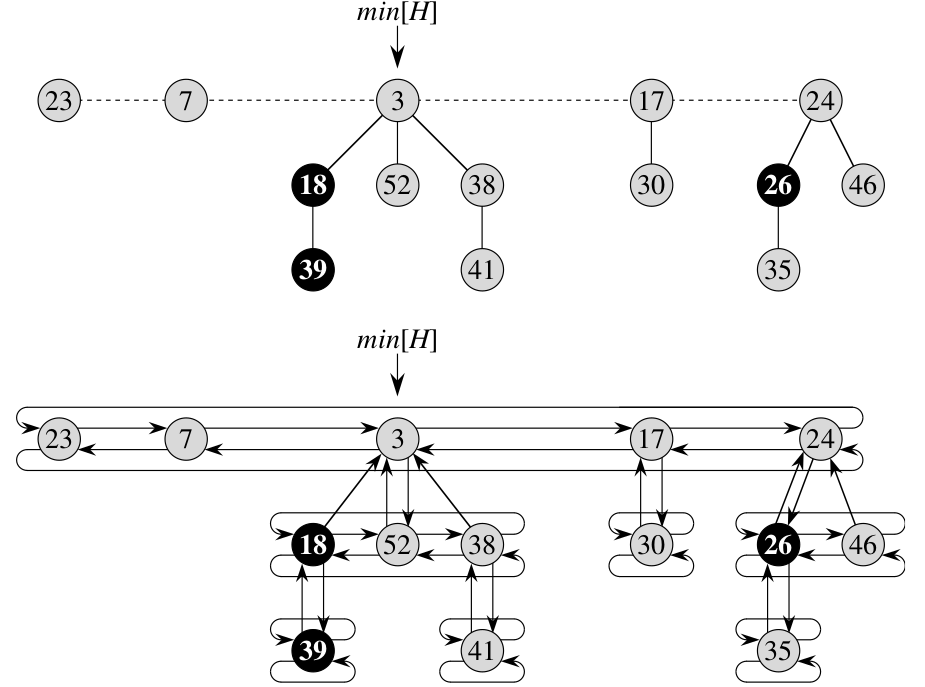
\includegraphics[width=.9\linewidth]{fibo}
\end{figure}

\framenote{Forrás: CLRS: Új algoritmusok 20.1~ábrája}
\end{frame}

\begin{frame}{Bináris vs. binomiális vs. Fibonacci kupac}
Kupacműveletek legrosszabb esetbeli viselkedése
\begin{table}
	\begin{tabular}{l|ccc}
		Művelet   &   Bináris   &   Binomiális  & Fibonacci\footnote{amortizált 
		költségek}   \\ \hline
		{\rmfamily\scshape Min-keres} & $O(1)$ &  $O(\log{n})$ & $O(1)$ \\
		{\rmfamily\scshape Sorbol-min} & $O(\log{n})$ &  $O(\log{n})$ & 
		$O(\log{n})$\\
		{\rmfamily\scshape Beszúr}    & $O(\log{n})$ & $O(\log n)$ 
		\footnote{amortizált költségben 
			$O(1)$} & $O(1)$\\
		{\rmfamily\scshape KulcsotCsökkent} & 	$O(\log{n})$ & $O(\log{n})$ & 
		$O(1)$\\
		{\rmfamily\scshape Egyesít} & $O(n)$ & $O(\log{n})$ & $O(1)$ \\
		{\rmfamily\scshape Töröl} & $O(\log{n})$ & $O(\log{n})$ & $O(\log{n})$
		\\
	\end{tabular}
\end{table}
\end{frame}

\begin{frame}{A Fibonacci kupacok viselkedése}
\begin{itemize}
	\item Remek választás, ha tudjuk, hogy a {\rmfamily\scshape Sorbol-min} és 
	{\rmfamily\scshape Töröl} műveleteket keveset használjuk
	\begin{itemize}
		\item Bizonyos gráfalgoritmusok (pl.~Dijkstra) esetében a 
		{\rmfamily\scshape KulcsotCsökkent} metódus alkalmazása dominál
	\end{itemize}
	\end{itemize}
\begin{alertblock}<2->{Ha nem hajtunk végre {\rmfamily\scshape KulcsotCsökkent} 
és {\rmfamily\scshape Töröl} műveletet}
	Egy (fokszám alapján) rendezetlen ''binomiális 
	kupacot'' kapunk \\
	$\rightarrow \log{n}$ a kupacbeli csúcsok maximális fokszámának 
	felső korlátja
\end{alertblock}
\begin{block}<3>{{\rmfamily\scshape KulcsotCsökkent} és {\rmfamily\scshape 
Töröl} műveletek végrehajtása esetén}
	$\log_\phi{n}=O(\log{n})$ a kupacbeli csúcsok 
	maximális fokszámának felső korlátja $\rightarrow$ innen jön a 
	Fibonacci-kupac elnevezés is (mivel az $i$-edik Fibonacci szám fölírható 
	$\frac{\phi^i-\psi^i}{\sqrt{5}}$ alakban, ahol $\phi=\frac{1+\sqrt{5}}{2}$)
\end{block}
\end{frame}

\begin{frame}{$O(1)$ idejű műveletek}
\begin{block}{{\rmfamily\scshape Egyesít} és {\rmfamily\scshape Beszúr}}
	$H_1$ és $H_2$ Fibonacci kupacok egyesítésekor a kupacok gyökérlistáit 
	összefűzzük, (min[H] aktualizálásán túl) \textbf{más teendőnk nincs}
\end{block}
\begin{block}{{\rmfamily\scshape Min-keres}}
	min[H] explicit tárolásából adódóan $O(1)$
\end{block}
\end{frame}

\begin{frame}{Minimális kulcs kivágása}
  \begin{itemize}
  	\item Ez az a pont, amikor próbáljuk a binomiális kupachoz hasonlóvá tenni 
  	a Fibonacci kupacunkat
  	\begin{enumerate}
  		\item min[H] által meghatározott csúcsot eltávolítjuk a gyökérlistából
  		\item min[H] gyerekeit a gyökérlistába delegáljuk
  		\item Összevonjuk a gyökérlistában szereplő azonos fokszámú fákat
  	\end{enumerate}
  \end{itemize}
\end{frame}

\begin{frame}{Kulcs értékének csökkentése}
	\begin{enumerate}
		\item Ha a kulcs csökkentett értéke túl kicsi, akkor a csúcsot kivágjuk 
		és a gyökérlistába helyezzük
		\item A kivágott csúcs szülejét (ha az nem gyökérlistabeli) megjelöltté 
		tesszük
		\item Amennyiben egy már megjelölt csúcs vesztené el egy újabb 
		gyerekét, úgy azt is rekurzívan a gyökérlistába visszük (megjelöltségét 
		eltávolítjuk)
	\end{enumerate}
\end{frame}

\begin{frame}{Összegzés}
\begin{itemize}
	\item Amortizált költségelemzéssel az adatszerkezetek hosszú távú 
	legrosszabb esetbeli viselkedését modellezhetjük
	\item Amortizált költségelemzés szempontjából a Fibonacci-kupac a megismert 
	leghatékonyabb kupac
	\item Egyes gráfalgoritmusok implementálásához kifejezetten hasznos 
	választás lehet
\end{itemize}
\end{frame}

\end{document}